\documentclass{scrreprt}

%Für deutsche Trennung
\usepackage[ngerman]{babel}
%Für UTF8-Codierung, mit Umlauten!
\usepackage[utf8]{inputenc}

%Für Links, auch innerhalb des Dokuments
\usepackage{hyperref}

%Einbinden von Grafiken
\usepackage{graphicx}

\usepackage{booktabs}

% Zusatzpakete verbatim und moreverb: listing-Umgebung
\usepackage{verbatim, moreverb}
\usepackage{color}
\definecolor{darkred}{rgb}{0.5,0,0}
\usepackage{listings}		%Für Quellcode

\lstloadlanguages{Java, XML}
\lstset{language=Java}
\lstset{
basicstyle=\ttfamily, % alle listings scriptsize drucken (kann man gerade noch lesen) und Schreibmaschinenschrift für alles
keywordstyle=\color{darkred}\bfseries, % Schlüsselwörter fett und dunkelrot drucken
commentstyle=\color{blue}, % Kommentare blau drucken
showstringspaces=false, % Strings im Code ohne Kenntlichmachung von Leerzeichen
breaklines=true,
frame=lines,
numbers=left,
numberstyle=\tiny,
tabsize=3
}

\newcommand{\lstx}[1]{\lstinline$#1$} 


\title{Software Quality Measurement}
\author{Gruppe H}
\date{\today}

\begin{document}

\maketitle
\tableofcontents

\chapter{Software Quality Measurement}

Für \lstx{mallet}\footnote{\href{https://github.com/mimno/Mallet}{Mallet af github}}, eine Verarbeitungssoftware für natürliche Sprache, sollen beispielhaft Kenngrößen für Softwarequalität ermittelt und ausgewertet werden. Zur Berechnung der Kenngrößen wird \lstx{ckjm}\footnote{\href{https://github.com/dspinellis/ckjm}{ckjm auf github},  \href{https://www.spinellis.gr/sw/ckjm/doc/indexw.html}{Manual}} verwendet, das alle sechs Kenngrößen nach Chidamber and Kemerer sowie zwei zusätzliche ermittelt. Die Ausgaben von \lstx{ckjm} werden mit Hilfe eines zur Verfügung gestellten, auf \lstx{matplotlib} basierenden Pythonskripts aufbereitet und in Form von Histogrammen dargestellt.

\begin{lstlisting}[caption = Beispiele für den Output von mallet]
cc.mallet.extract.test.TestDocumentExtraction 7 0 0 20 31 21 0 7
cc.mallet.pipe.SerialPipes$Predicate 2 1 0 2 3 1 1 2
cc.mallet.classify.BalancedWinnowTrainer 6 0 0 11 21 11 1 6
cc.mallet.util.CharSequenceLexer 20 1 0 1 45 94 14 16
...
\end{lstlisting}


%TODO Output the 3 classes with the highest and lowest scores for the measures CBO and LCOM. (You may use the provided file findExtremes.py for doing this) Have a look at those classes, why do they have high/low scores for CBO and LCOM? How do you judge the quality of the classes and the effectiveness of the measures? Write a short explanation. 

\section{CBO – Kopplung ziwschen Objektklassen}
CBO 
CBO: Coupling between object classes

\begin{figure}
 \centering
 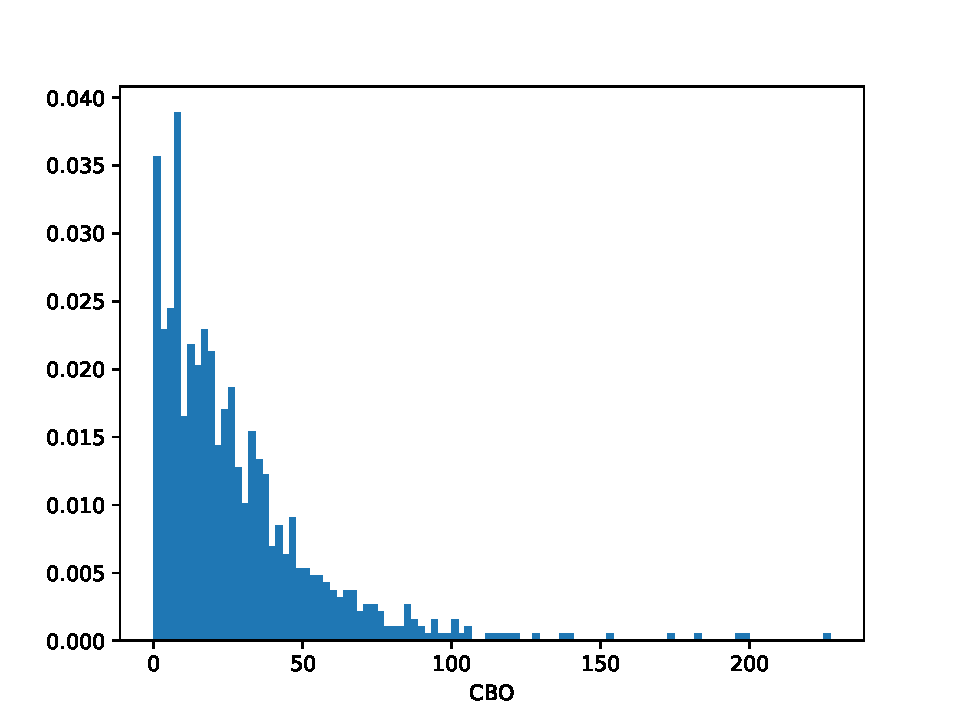
\includegraphics[width=.8\textwidth]{./CBO.pdf}
 % CBO.pdf: 0x0 pixel, 300dpi, 0.00x0.00 cm, bb=
 \caption{Coupling of Object Classes}
 \label{abb:cbo}
\end{figure}


\begin{center}
\begin{tabular}{ll}
\toprule
CBO: schlechteste Klassen\\
\midrule
\lstx{cc.mallet.optimize.OptimizerEvaluator} & 0\\
\lstx{cc.mallet.util.tests.TestAStar\$1} & 0\\
\lstx{cc.mallet.pipe.CharSequenceRemoveHTML\$1} & 0 \\
\bottomrule
\end{tabular}
\end{center}


\begin{center}
\begin{tabular}{ll}
\toprule
CBO: beste Klassen\\
\midrule
\lstx{cc.mallet.topics.ParallelTopicModel} & 227 \\
\lstx{cc.mallet.fst.tests.TestCRF} & 198\\
 \lstx{cc.mallet.topics.LDAHyper}&196 \\
\bottomrule
\end{tabular}
\end{center}


Ein hoher Wert des CBO ist erwünscht. Das bedeutet, dass Methoden mit vielen Instanzvariablen eng gekoppelt sind, was sich wiederum positiv auf die Softwarequalität auswirkt.

Ein kleiner Wert ist unerwünscht, da solche Klassen nicht mit anderen Klassen zusammen wirken.

\section{LCOM – Mangel an Abgeschlossenheit}

LCOM
LCOM: Lack of cohesion in methods

\begin{figure}
 \centering
 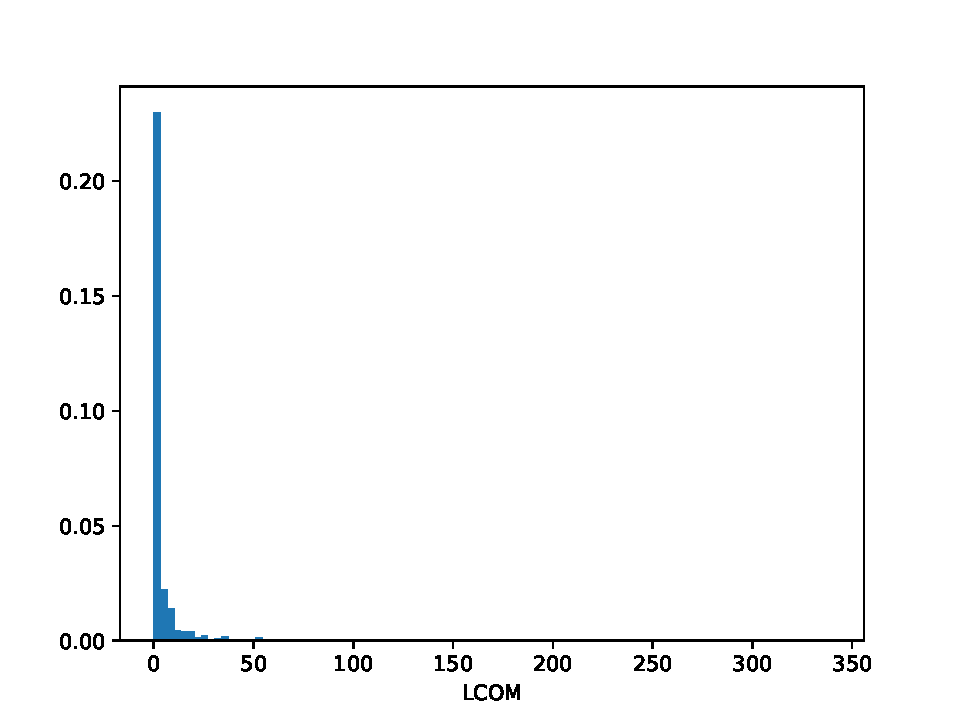
\includegraphics[width=.8\textwidth]{./LCOM.pdf}
 % LCOM.pdf: 0x0 pixel, 300dpi, 0.00x0.00 cm, bb=
 \caption{Lack of Cohesion}
 \label{abb:lcom}
\end{figure}


\begin{center}
\begin{tabular}{ll}
\toprule
LCOM: beste Klassen\\
\midrule
\lstx{cc.mallet.extract.test.TestDocumentExtraction} &0 \\
\lstx{cc.mallet.fst.LabelDistributionEvaluator} &0 \\
\lstx{cc.mallet.optimize.OptimizerEvaluator\$ByBatchGradient} &0  \\
\bottomrule
\end{tabular}
\end{center}


\begin{center}
\begin{tabular}{ll}
\toprule
LCOM: schlechteste Klassen \\
\midrule
\lstx{cc.mallet.pipe.Pipe} & 229\\
\lstx{cc.mallet.types.InstanceList} & 241\\
\lstx{cc.mallet.types.Instance} & 339 \\
\bottomrule
\end{tabular}
\end{center}

Und hier ist es dann halt andersrum.

Der LCOM-Wert drückt den Mangel an Kohäsion aus, das heißt dem Zusammenhang zwischen den Methoden. Ein großer Wert ist hier schlecht.

\section{Weitere Kenngrößen und graphische Darstellung}

%TODO 7. Plot a histogram for each of the measures using matplotlib. (You may use the provided file findExtremes.py for doing this) What insights do you gain from these plots concerning the Mallet repository? You may compare the repository to other repositories of your choosing.

Die Kenngrößen werden als normierte Histogramme dargestellt, auf der x-Achse sind Bereiche möglicher Werte der Kenngröße aufgetragen, auf der y-Achse der Anteil der Klassen, die diesem Wertebereich zugeordnet sind.

Als weitere Kenngrößen würden von \lstx{ckjm} ermittelt:

\begin{itemize}
\item WMC: Weighted methods per class
\item DIT: Depth of Inheritance Tree
\item NOC: Number of Children
\item RFC: Response for a Class
\item Ca: Afferent coupling (not a C\&K metric)
\item NPM: Number of Public Methods for a class (not a C\&K metric)
\end{itemize}

\begin{figure}
 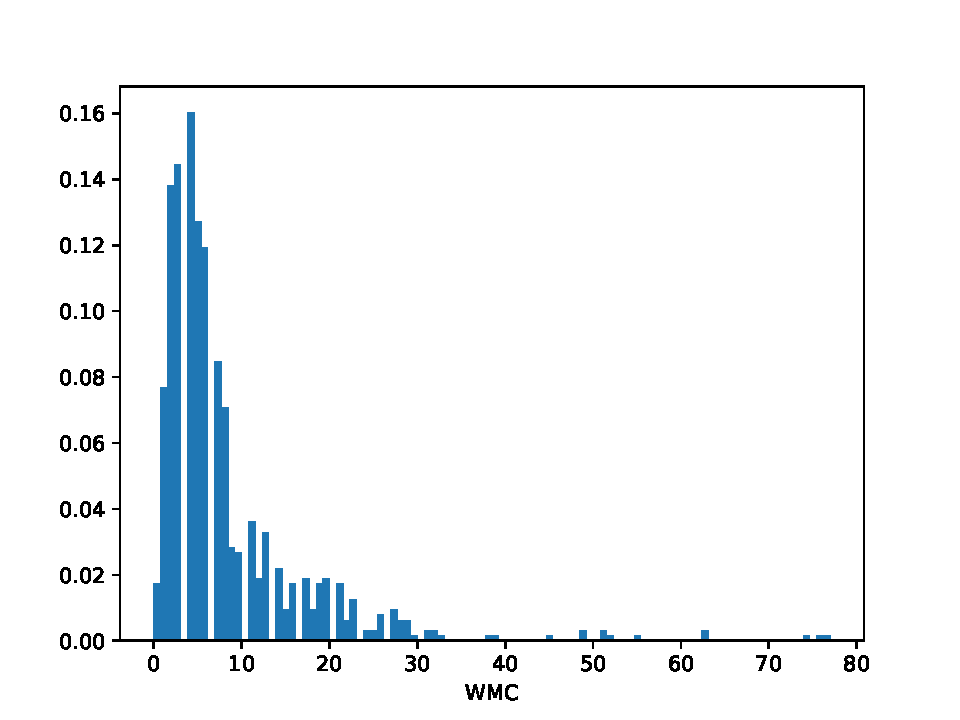
\includegraphics[width=.45\textwidth]{./WMC.pdf}
 % WMC.pdf: 0x0 pixel, 300dpi, 0.00x0.00 cm, bb=
  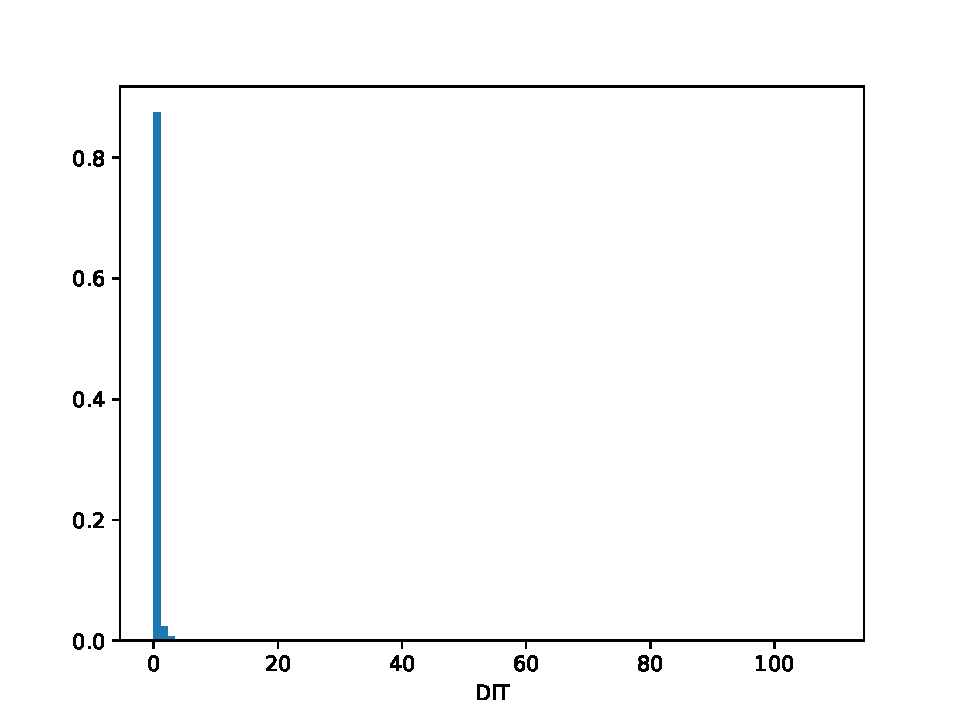
\includegraphics[width=.45\textwidth]{./DIT.pdf}
 \caption{WMC und DIT}
 \label{abb:wmc}
\end{figure}

% Depth of inheritance tree (DIT)
% This represents the number of discrete levels in the inheritance tree where
% subclasses inherit attributes and operations (methods) from superclasses. The
% deeper the inheritance tree, the more complex the design. Many object classes
% may have to be understood to understand the object classes at the leaves of the
% tree.

\begin{figure}
 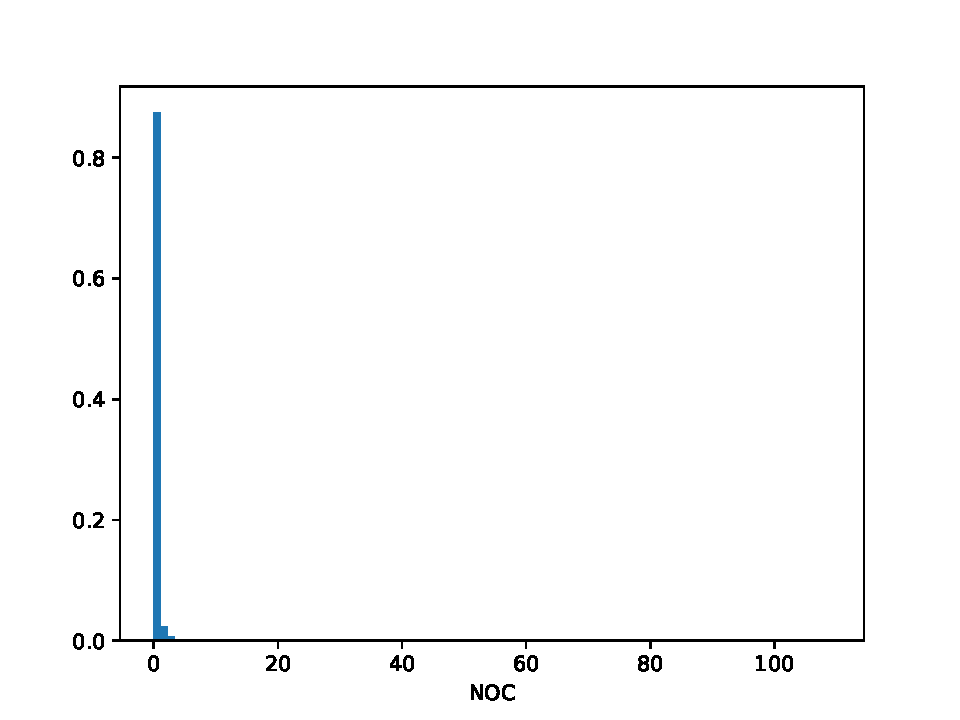
\includegraphics[width=.45\textwidth]{./NOC.pdf}
 % WMC.pdf: 0x0 pixel, 300dpi, 0.00x0.00 cm, bb=
  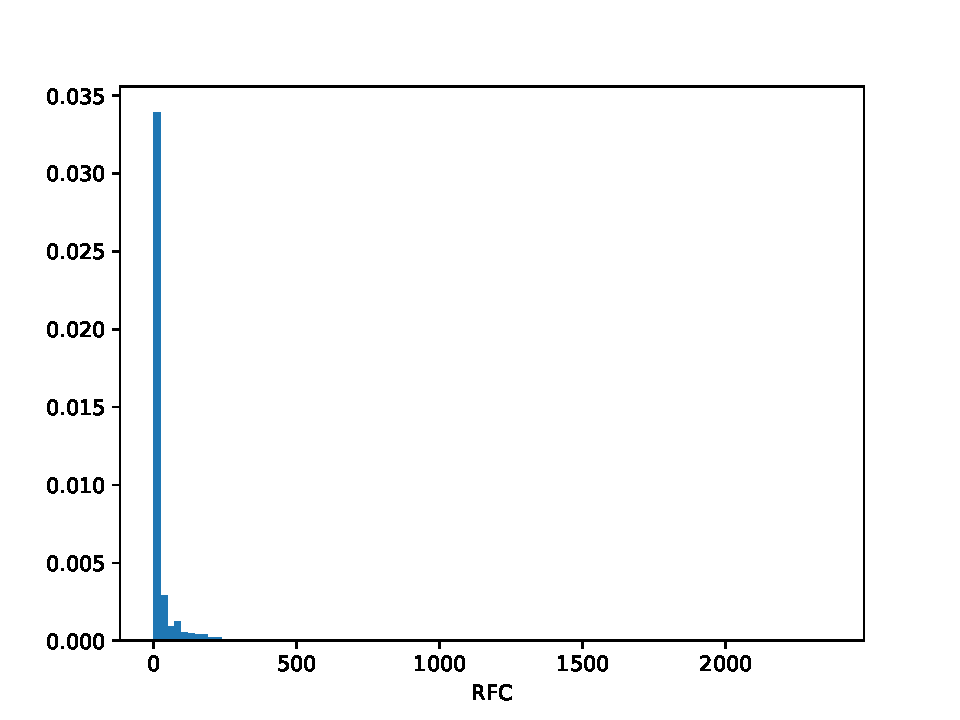
\includegraphics[width=.45\textwidth]{./RFC.pdf}
 \caption{NOC und RFC}
 \label{abb:noc_rfc}
\end{figure}

% Number of children (NOC)
% This is a measure of the number of immediate subclasses in a class. It measures
% the breadth of a class hierarchy, whereas DIT measures its depth. A high value
% for NOC may indicate greater reuse. It may mean that more effort should be
% made in validating base classes because of the number of subclasses that
% depend on them.

\begin{figure}
 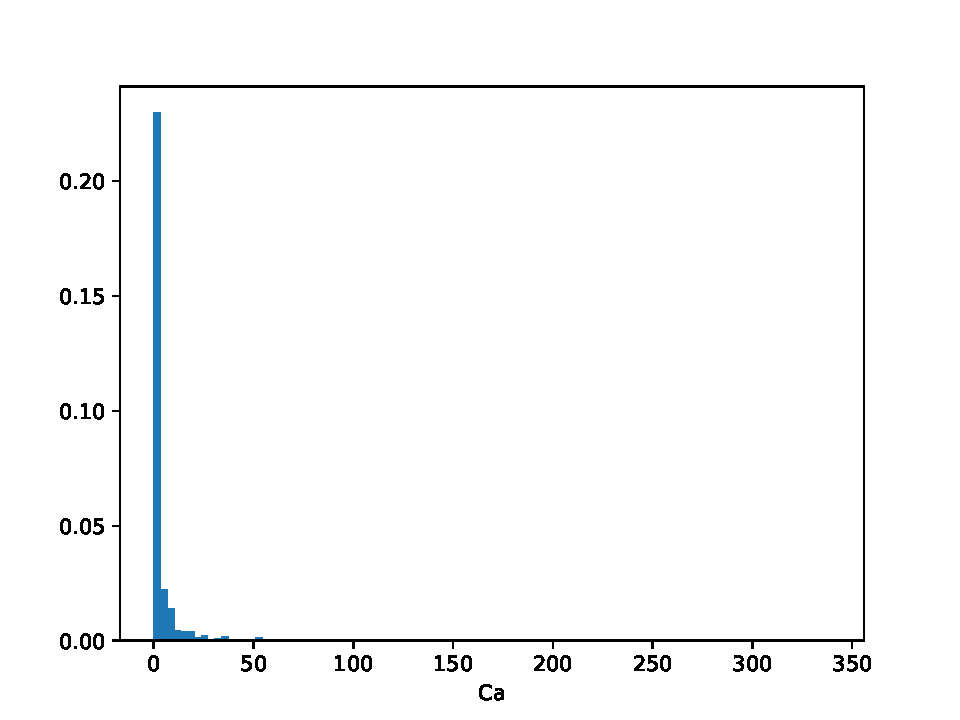
\includegraphics[width=.45\textwidth]{./Ca.pdf}
 % WMC.pdf: 0x0 pixel, 300dpi, 0.00x0.00 cm, bb=
  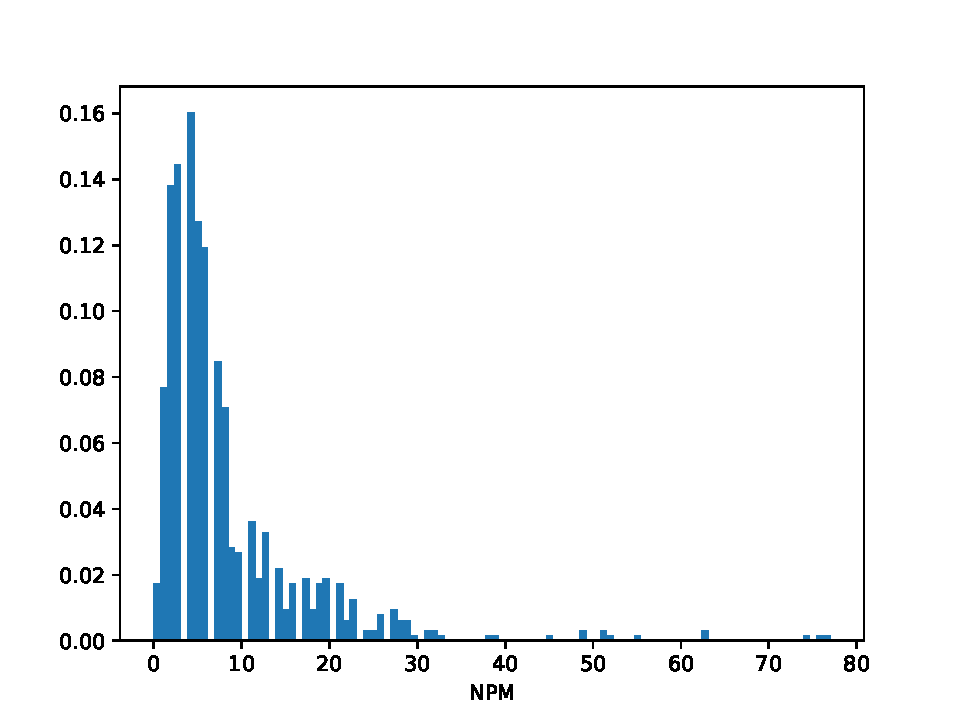
\includegraphics[width=.45\textwidth]{./NPM.pdf}
 \caption{Ca und NPM}
 \label{abb:ca_npm}
\end{figure}

\section{Vergleich mit einer abgeänderten Version von mallet}

Dem Programm \lstx{mallet} werden zwei weitere Klassen \lstx{NewParallelTopicModel.java} und \lstx{TopicInferencerInterface.java} hinzugefügt. Nach dem Kompilieren wird die Analyse von \lstx{mallet} wiederholt und es werden die Kennzahlen der Klassen \lstx{NewParallelTopicModel} und \lstx{ParallelTopicModel} verglichen:

%TODO 8. In the package cc.mallet.topics there is a class called ParallelTopicModel which is used to learn a model on some data. A different class in the same package, called TopicInferencer, is used for the evaluation of the trained model. Add the provided Java files to this package and rebuild Mallet. Now compare the output of CKJM on ParallelTopicModel and NewParallelTopicModel. What do the new values indicate? What is the difference between the two classes?

\begin{tabular}{lllllllll}
\toprule
Klasse & WMC & DIT & NOC & CBO & RFC & LCOM & Ce & NPM \\
\midrule
\lstx{NewParallelTopicModel} & 68 & 1 & 0 & 22 & 233 & 800 & 0 & 61 \\
\lstx{ParallelTopicModel} & 63 & 1 & 2 & 21 & 227 & 627 & 11 & 58 \\
\bottomrule
\end{tabular}



\end{document}
